\chapter{Results}

To test the cross-validation (CV) approach to error estimation this code has been added into the \cite{Uieda2016} synthetic-crust1 with Moho depth information extracted from the CRUST1.0 model \citep{Laske2013}. As previously mentioned this procedure needs the availability of seismic point estimates, the data for this is from Assumpção et al. (2013). These Moho depth estimates along with their geographical location can be seen in Figure~\ref{fig:seismic_locations} and in total there are 937 points.
The cross-validation approach used is repeated random sub-sample validation and as mentioned in the methodology randomly splits the full seismic data set into a training and testing (validating) set, with the training set compared to the solution to attain cross-validation values, the best solution is then selected from the smallest cross-validation value which is then scored against the testing set to attain the Mean Square Errors and subsequently the square root of these values which are the difference between the model and the point estimates. This error gives an indication to the average uncertainty in the overall model depth, and mainly to how good the model is where seismic data is not present which is largely the case for South America as most seismic point estimates are situated near the coast.
\section{Cross-validation results from the synthetic model}
In this run, the seismic point data will be split into a training and testing set, for a range of different proportions, these include the training size being 2/3, 3/4, and finally 4/5 of the full data. For each training size, the data that makes up this subset will be selected randomly from the full set for 100 iterations. The remaining data that was not selected for each iteration will be put into the validating set and held back for later scoring. As there are 937 separate seismic point estimates when the data is split these proportions need to be rounded to the nearest integer hence 2/3 is 625 data points, 3/4 is 703 points, and finally 4/5 rounds to 750 points. Figure~\ref{fig:histogram_no_intrusion}
\begin{figure}[h]
  \begin{center}
    % Width can be set to particular size (10cm) or relative to the page size,
    % like 0.5\textwidth (for half page) or \textwidth (for full page).
    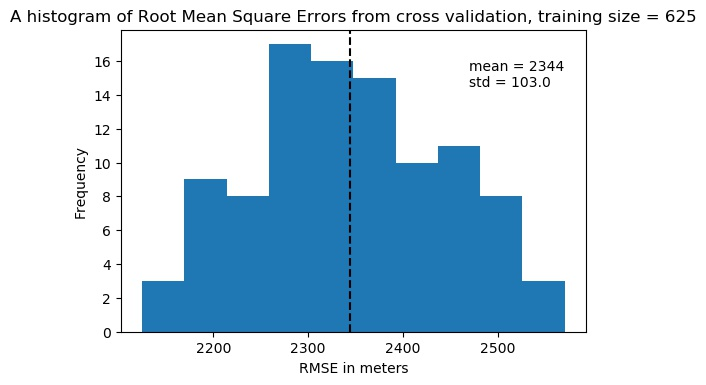
\includegraphics[width=0.6\textwidth]{figures/no-intrusion-625}
    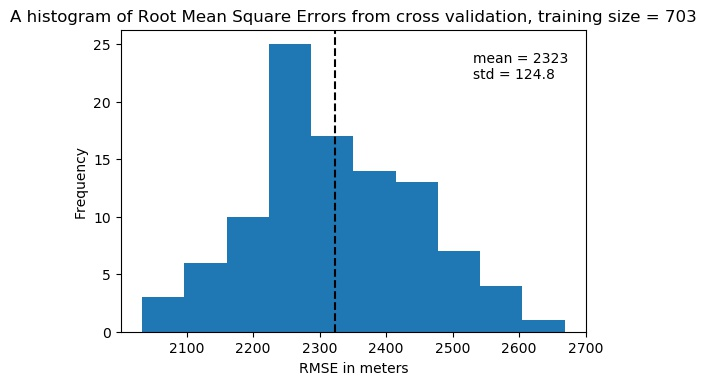
\includegraphics[width=0.6\textwidth]{figures/no-intrusion-703}
    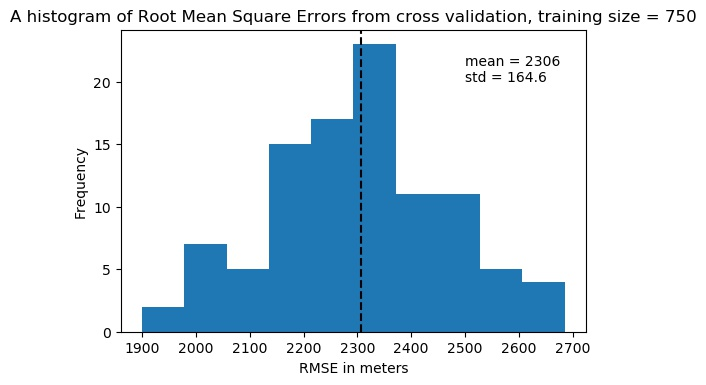
\includegraphics[width=0.6\textwidth]{figures/no-intrusion-750}
  \end{center}
  \caption{
   RMS values from cross validation. Training sizes top to bottom are: 625, 703, and 750 all have 100 iterations. The dotted black line indicates the mean RMS value which is stated in the top right corner along with the standard deviation (std).
  }
  % Label used to reference the figure in the text.
  \label{fig:histogram_no_intrusion}
\end{figure}
shows the results of the cross-validation in the form of histograms showing the RMS values for all the iterations. All of these display somewhat of a normal distribution that should be more profound if more iterations were run. The mean values for all these histograms are very similar with all the values ranging between 2300-2350 metres with the highest value, 2344m, associated with the smallest training size of 625 and the smallest RMS value correlating to the largest training size. The standard deviation (std), which is a measure of the tightness of the spread to the mean value, increases with larger training sizes. This means that for larger training sizes the RMS values are more spread out with points for the largest training size of 750 having values that range from 1900-2700m with a standard deviation of 164.6. On the other hand, the other two sizes, 625 and 703, have std values of 103.0 and 124.8 respectively with RMS values not reaching below 2000m.
\cite{Szwillus2019} uses a similar method of cross-validation to estimate Moho uncertainty, except the method used is seismic interpolation and is on a global scale rather than just South America Figure~\ref{fig:uncertainty}.
\begin{figure}[h]
  \begin{center}
    % Width can be set to particular size (10cm) or relative to the page size,
    % like 0.5\textwidth (for half page) or \textwidth (for full page).
    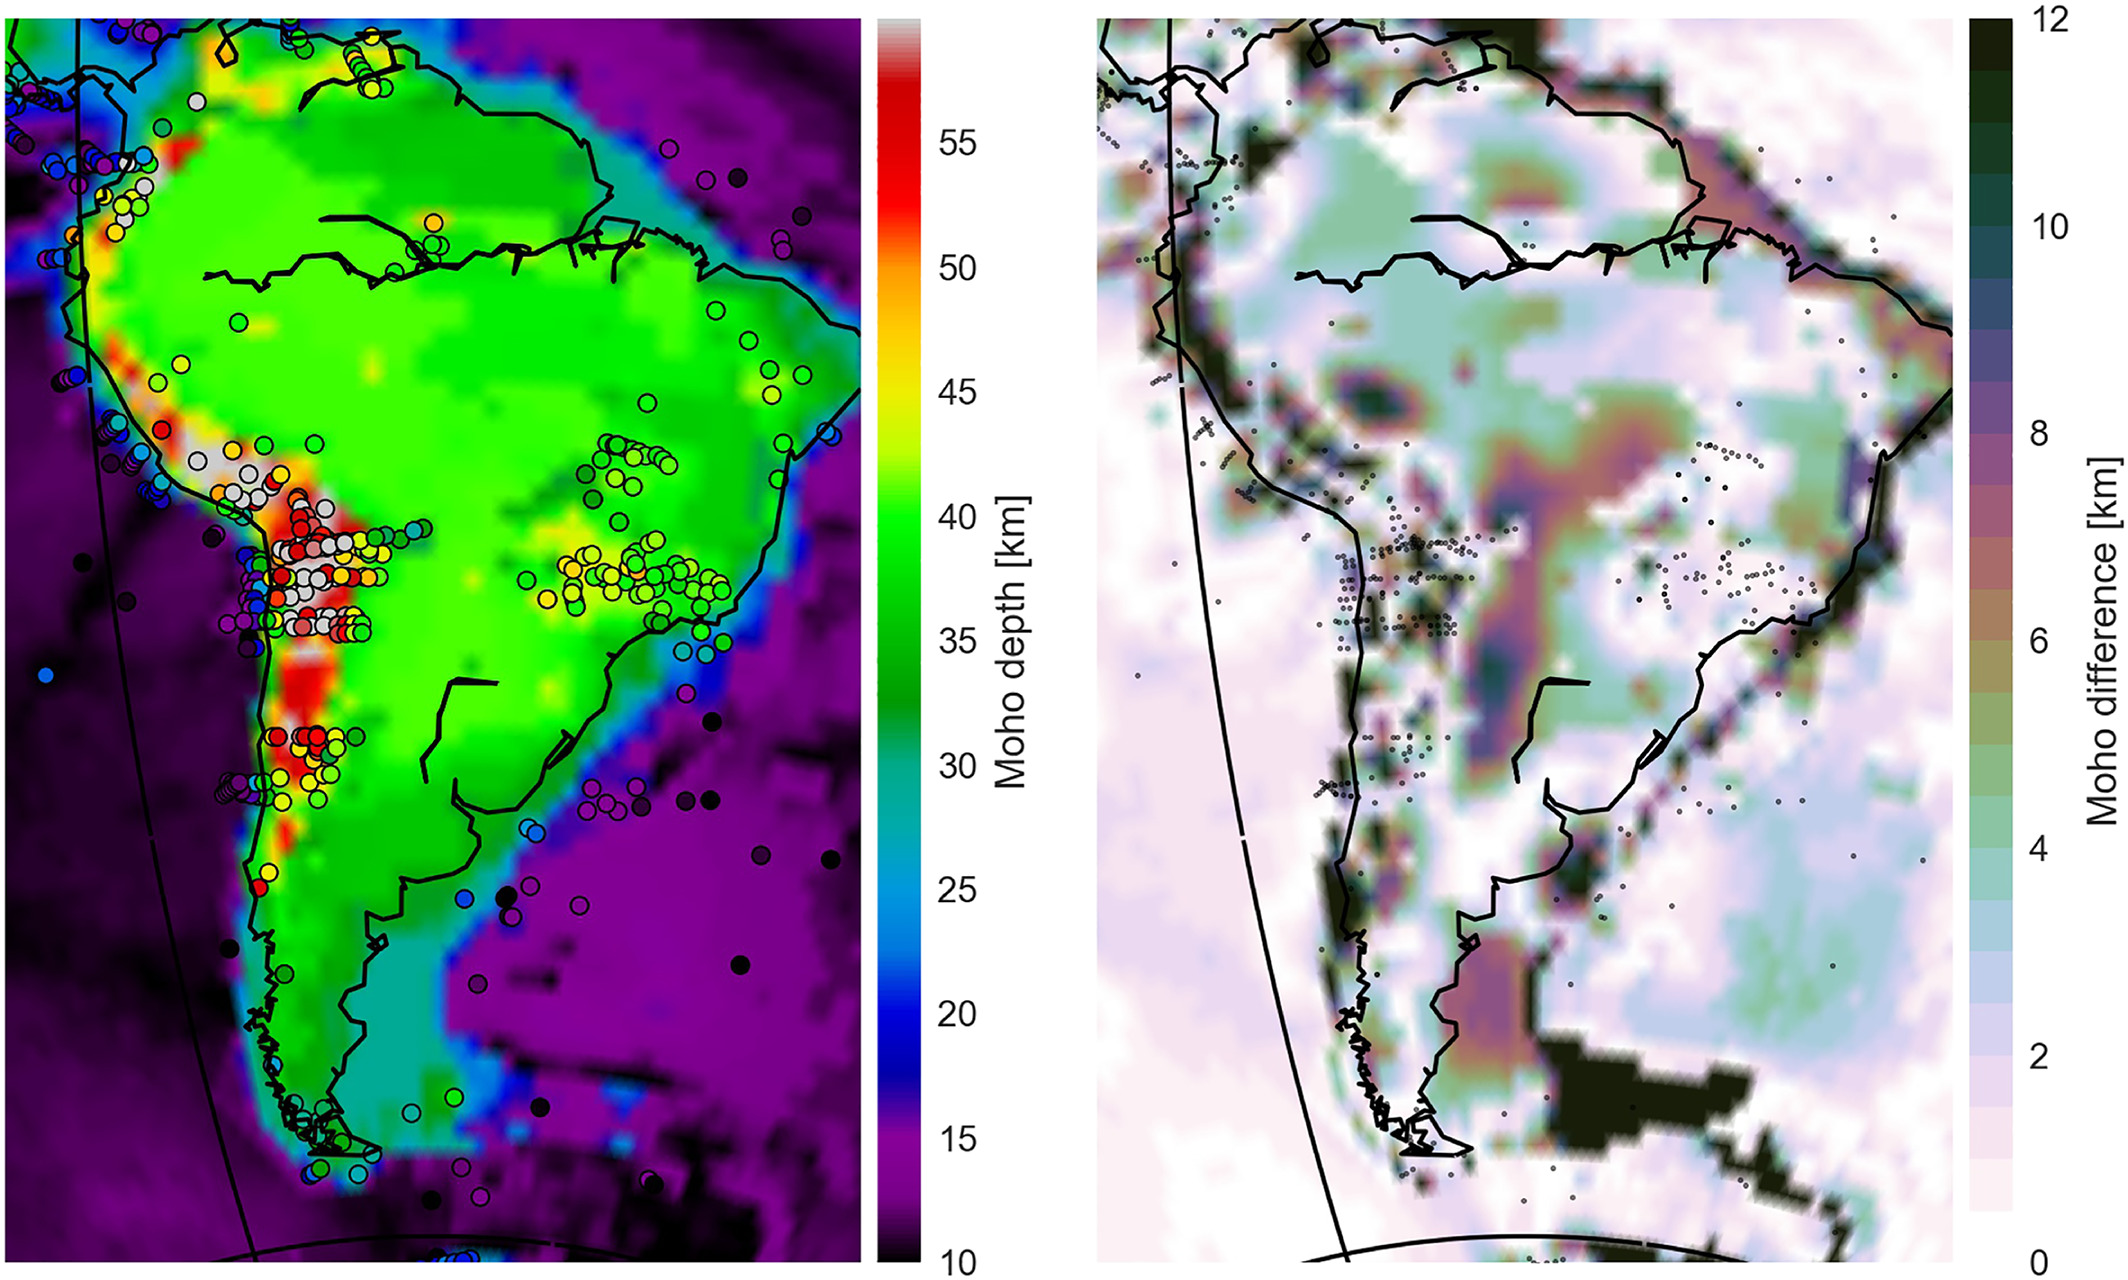
\includegraphics[width=0.9\textwidth]{figures/Szwillus-uncertainty}
  \end{center}
  \caption{
   Interpolated Moho depth and the corresponding uncertainty values for South America. After \cite{Szwillus2019}.
  }
  % Label used to reference the figure in the text.
  \label{fig:uncertainty}
\end{figure}
The average Moho uncertainty calculated was 4.5km for South America however, the range of values was much larger with uncertainties in some places reaching 12km although these values were in places where no seismic data was present. This result is just over 2km higher than the mean uncertainty values seen in the histograms of around 2.3-2.4km and is likely due to the differing method.
However, when compared to the model, these RMS values are quite small in comparison to the Moho depths from the model which on average is probably between 30-40km across the continent, where most of the seismic point estimates are located. The difference between the individual point estimates and the model in that location is shown in Figure~\ref{fig:difference_no_intrusion}.
\begin{figure}[h]
  \begin{center}
    % Width can be set to particular size (10cm) or relative to the page size,
    % like 0.5\textwidth (for half page) or \textwidth (for full page).
    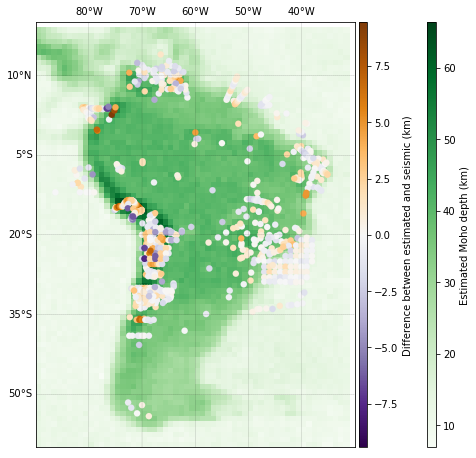
\includegraphics[width=0.9\textwidth]{figures/difference-no-intrusion}
  \end{center}
  \caption{
   Plot of estimated Moho depth without the added underplating with seismic point estimates superimposed. The colours of the point estimates (circles) represent the difference between the model and the seismic data.
  }
  % Label used to reference the figure in the text.
  \label{fig:difference_no_intrusion}
\end{figure}
The point estimates generally tend to agree with the model, however, in few places like the Andes the model is underpredicting the Moho depth when compared to the point estimates, this could have given rise to the higher standard deviation for the larger training sets as a majority of the points held back for the validating set for some iterations may have been points from the Andes. This is especially likely seeing as a reasonable proportion of the full 937 points are situated in the mountain range.
\section{Cross-validation results after adding in underplating}
This trial run is identical in every way to the synthetic-crust1 model except an intrusion has been added in the Paraná Basin. There are clusters of seismic point estimates situated in the same and surrounding area. Like the synthetic model the training sizes are 625, 703 and 750 with the full data set consisting of 937 points, each size was run with 100 iterations to create histograms of RMS values shown in Figure~\ref{fig:histogram_intrusion}.
\begin{figure}[h]
  \begin{center}
    % Width can be set to particular size (10cm) or relative to the page size,
    % like 0.5\textwidth (for half page) or \textwidth (for full page).
    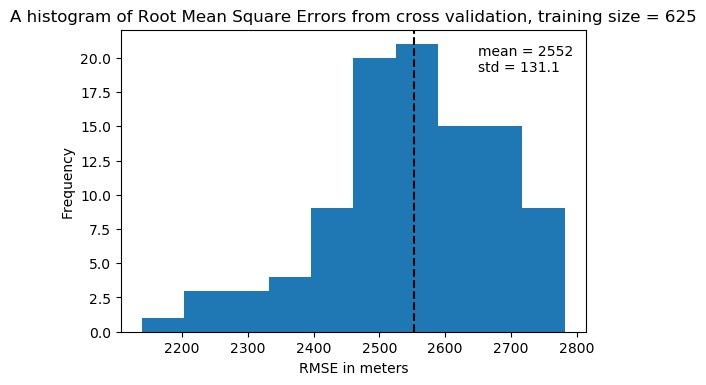
\includegraphics[width=0.6\textwidth]{figures/intrusion-625}
    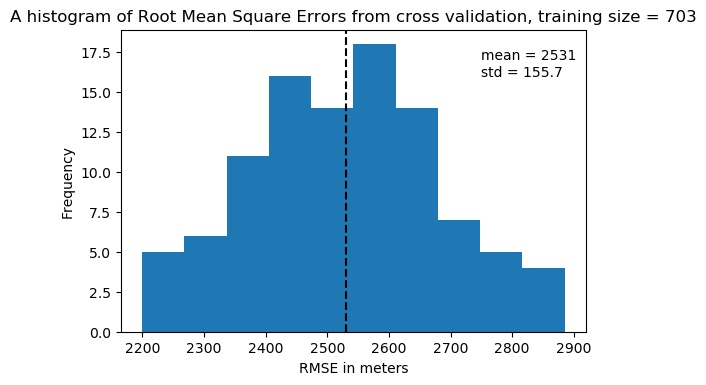
\includegraphics[width=0.6\textwidth]{figures/intrusion-703}
    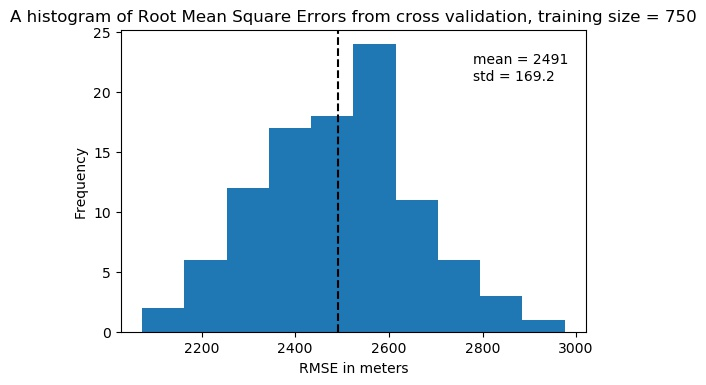
\includegraphics[width=0.6\textwidth]{figures/intrusion-750}
  \end{center}
  \caption{
   RMS values from cross validation with Paraná Basin underplating included in the model. Training sizes top to bottom are: 625, 703, and 750 all have 100 iterations. The dotted black line indicates the mean RMS value which is stated in the top right corner along with the standard deviation (std).
  }
  % Label used to reference the figure in the text.
  \label{fig:histogram_intrusion}
\end{figure}
These histograms like those without the intrusion display a fairly normal distribution, however, the mean values are higher. This result was expected as the inclusion of the underplating will increase the difference in that area between the model and seismic point estimates. The mean values of each training size are 2552m, 2531m and 2491m respectively with the value decreasing as the training size increases, these are around 200m higher than the equivalent training size without the intrusion. Like the results of the model without the intrusion too the standard deviation increases with larger training sizes. In comparison, these standard deviations are higher with the std value for size 625 being 131.1 which is around 28m higher than its counterpart. The ranges of the RMS values though do not exceed 1900-2700m the higher std values are explained by a larger proportion of the values attained through cross-validation being near the edges of the range.
These results in comparison to the overall Moho depths are not that large as again the depths of the model are very similar to that of the model without the intrusion with the mean value being somewhere between 30-40km, so an error of about 2.5km or around 6-8\%. This error is low and so indicates that the model fits the seismic data very well. These discrepancies may in part be due to the Andes problem stated above but also to the large difference between the model and the point estimates in the Paraná Basin meaning that if the majority of these points with large disparities (see Figure~\ref{difference}) are selected as part of the testing set then the RMS value increases.
\begin{figure}[h]
  \begin{center}
    % Width can be set to particular size (10cm) or relative to the page size,
    % like 0.5\textwidth (for half page) or \textwidth (for full page).
    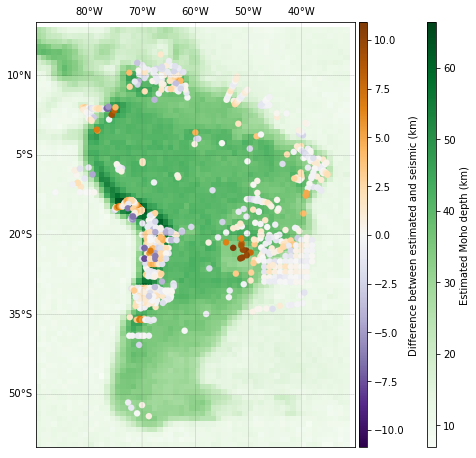
\includegraphics[width=0.9\textwidth]{figures/difference}
  \end{center}
  \caption{
   Plot of estimated Moho depth with the added underplating with seismic point estimates superimposed. The colours of the point estimates (circles) represent the difference between the model and the seismic data.
  }
  % Label used to reference the figure in the text.
  \label{fig:difference}
\end{figure}
\section{Software and run times}
For the code with and without the intrusion added both took 1hr and 57 minutes with 3 different training sizes and 100 iterations per individual size, i.e. 300 iterations in total. This was performed on a laptop computer with an AMD Ryzen 5 3500U 2.1GHz processor.